\documentclass{article}

\usepackage{fancyhdr}
\usepackage{lastpage}
\usepackage{extramarks}
\usepackage[usenames,dvipsnames]{color}
\usepackage{amsmath}
\usepackage{amsthm}
\usepackage{amsfonts}
\usepackage{changepage}
\usepackage{lineno}
\usepackage[plain]{algorithm}
\usepackage{algpseudocode}
\usepackage{tikz}
\usepackage{hyperref}

\usetikzlibrary{arrows}
\usetikzlibrary{positioning}

\topmargin=-0.45in
\evensidemargin=0in
\oddsidemargin=0in
\textwidth=6.5in
\textheight=9.0in
\headsep=0.25in

\linespread{1.1}

\pagestyle{fancy}
\lhead{\hmwkAuthorName}
\chead{\hmwkClass\ (\hmwkClassInstructor\ \hmwkClassTime): \hmwkTitle}
\rhead{\firstxmark}
\lfoot{\lastxmark}
\cfoot{}

\renewcommand\headrulewidth{0.4pt}
\renewcommand\footrulewidth{0.4pt}

\setlength{\floatsep}{100pt}
\renewcommand{\algorithmicrequire}{\textbf{Input:}}
\renewcommand{\algorithmicensure}{\textbf{Output:}}

\setlength\parindent{0pt}

\hypersetup{colorlinks=true}

\newcommand{\enterProblemHeader}[1]{
    \nobreak\extramarks{}{Problem \arabic{#1} continued on next page\ldots}\nobreak{}
    \nobreak\extramarks{Problem \arabic{#1} (continued)}{Problem \arabic{#1} continued on next page\ldots}\nobreak{}
}

\newcommand{\exitProblemHeader}[1]{
    \nobreak\extramarks{Problem \arabic{#1} (continued)}{Problem \arabic{#1} continued on next page\ldots}\nobreak{}
    \stepcounter{#1}
    \nobreak\extramarks{Problem \arabic{#1}}{}\nobreak{}
}

\setcounter{secnumdepth}{0}
\newcounter{homeworkProblemCounter}
\setcounter{homeworkProblemCounter}{1}
\nobreak\extramarks{Problem \arabic{homeworkProblemCounter}}{}\nobreak{}

\newenvironment{homeworkProblem}{
    \section{Problem \arabic{homeworkProblemCounter}}
    \enterProblemHeader{homeworkProblemCounter}
}{
    \exitProblemHeader{homeworkProblemCounter}
}

\newcommand{\hmwkTitle}{Homework\ \#5}
\newcommand{\hmwkDueDate}{November 11, 2013 at 4:30pm}
\newcommand{\hmwkClass}{CS311}
\newcommand{\hmwkClassTime}{Section 3}
\newcommand{\hmwkClassInstructor}{Professor Lathrop}
\newcommand{\hmwkAuthorName}{Josh Davis}
\newcommand{\solution}{{\large \bfseries Solution}}

\title{
    \vspace{2in}
    \textmd{\textbf{\hmwkClass:\ \hmwkTitle}}\\
    \normalsize\vspace{0.1in}\small{Due\ on\ \hmwkDueDate}\\
    \vspace{0.1in}\large{\textit{\hmwkClassInstructor\ \hmwkClassTime}}
    \vspace{3in}
}

\author{\textbf{\hmwkAuthorName}}
\date{}

\newcommand{\alg}[1]{\textsc{\bfseries \footnotesize #1}}

\begin{document}

\maketitle

\pagebreak

\begin{homeworkProblem}
    Give algorithms for the following operations.
    \\

    \solution

    Algorithms for each part are below.
    \\

    \textbf{Part A}

    Give an algorithm that multiples two degree-1 polynomials with only three
    multiply operations.
    \\

    \begin{algorithm}[]
        \begin{algorithmic}[1]
            \Function{MultiplySingleDegreePolynomials}{$a, b, c, d$}
            \State{} \Return{$0$}
            \EndFunction{}
        \end{algorithmic}
        \caption{Multiply 1 degree polynomial}
    \end{algorithm}

    \textbf{Part B}

    Give a divide-and-conquer algorithm for multiplying two polynomials of
    degree \(n\). Prove using the master theorem that your algorithm runs in
    \(\Theta(n^{\log_2 3})\). You may assume that \(n + 1\) is a power of 2.
    \\

    \begin{algorithm}[]
        \begin{algorithmic}[1]
            \Function{MultiplyNDegreePolynomials}{}
            \State{} \Return{$0$}
            \EndFunction{}
        \end{algorithmic}
        \caption{Multiply \(n\) degree polynomial}
    \end{algorithm}
\end{homeworkProblem}

\pagebreak

\begin{homeworkProblem}
    Give an \(O(\log n)\) time algorithm that computes the following function:
    \\

    \alg{MEDIAN-OF-TWO($l_1, l_2$)}

    \begin{algorithm}[]
        \begin{algorithmic}[1]
            \Require \(l_1\) and \(l_2\) are two sorted lists of integers. Each
            list has \(n\) elements (\(2n\) elements in total) and the value of
            each element in the lists is unique.

            \Ensure The value of the \(n^{th}\) smallest integer in the set of
            \(2n\) integers is \(l_1\) and \(l_2\).
        \end{algorithmic}
    \end{algorithm}

    \solution

    \begin{algorithm}[]
        \begin{algorithmic}[1]
            \Function{Mid}{$x, y$}
                \State{} \Return{$(y - x) / 2 + x$}
            \EndFunction{}
            \\
            \Function{Median-Of-Two}{$l_1, l_2$}
                \State{} $start1 \gets 0$
                \State{} $start2 \gets 0$
                \State{} $end1 \gets l_1.length$
                \State{} $end2 \gets l_2.length$
                \State{} $mid1 \gets \Call{Mid}{start1, end1}$
                \State{} $mid2 \gets \Call{Mid}{start2, end2}$
                \\
                \While{$mid1 < end1$ and $mid2 < e2$}
                    \If{$l1[mid1] < l2[mid2]$}
                        \State{} $start1 \gets mid1$
                        \State{} $end2 \gets mid2$
                    \Else{}
                        \State{} $end1 \gets mid1$
                        \State{} $start2 \gets mid2$
                    \EndIf
                    \\
                    \State{} $mid1 \gets \Call{Mid}{start1, end1}$
                    \State{} $mid2 \gets \Call{Mid}{start2, end2}$
                \EndWhile
                \\
                \If{$mid1 \geq end1$}
                    \State{} \Return{$l1[mid1]$}
                \Else{}
                    \State{} \Return{$l2[mid2]$}
                \EndIf
            \EndFunction{}
        \end{algorithmic}
        \caption{Value of the \(n^{th}\) smallest integer in either list}
    \end{algorithm}
\end{homeworkProblem}

\pagebreak

\begin{homeworkProblem}
    Give an \(O(n)\) average case running time algorithm that computes the
    following:
    \\

    \alg{Kth-SMALLEST($list, k$)}

    \begin{algorithm}[]
        \begin{algorithmic}[1]
            \Require An unsorted list \(list\) of unique integers and an integer \(k\)

            \Ensure The value of the \(k^{th}\) smallest integer from the list
        \end{algorithmic}
    \end{algorithm}

    \solution

    The algorithm is based off of \alg{QuickSort} and is often called
    \alg{QuickSelect}\(^{[1]}\).  The principle idea is to use the partitioning function
    of \alg{QuickSort} because the element that is selected to be a partition
    will be placed in its correct place in the list. The position then will tell
    us where to look for the \(k\)th item.

    \begin{algorithm}[]
        \begin{algorithmic}[1]
            \Function{Kth-SMALLEST}{$list, k$}
                \State{} $index \gets \Call{Kth-SMALLEST-REC}{list, k, 0, list.length}$
                \State{} \Return{$list[index]$}
            \EndFunction{}
            \\
            \Function{QuickSelect}{$list, k, start, end$}
                \If{$start \geq end$}
                    \State{} \Return{$end$}
                \EndIf{}
                \\
                \State{} $partition \gets \Call{Partition}{list, k, start, end}$
                \\
                \If{$k < partition$}
                    \State{} \Return{} \Call{QuickSelect}{$list, start, partition - 1$}
                \ElsIf{$k > partition$}
                    \State{} \Return{} \Call{QuickSelect}{$list, partition + 1, end$}
                \EndIf{}
                \\
                \State{} \Return{$list[k]$}
            \EndFunction{}
        \end{algorithmic}
        \caption{Give the $k^{th}$ smallest integer from the list}
    \end{algorithm}

    Where the \alg{Partition} algorithm is dependent on the type of
    partitioning scheme used.
    \\

    \textbf{Reference}

    \([1]\) Tim Roughgarden's lecture on Coursera.org:
    \url{https://class.coursera.org/algo-004/lecture/36}
\end{homeworkProblem}

\pagebreak

\begin{homeworkProblem}
    Let \(T\) be a tree with \(n\) vertices. We say that a vertex \(v\) is a
    \textit{minimal separator of T} if its removal splits \(T\) into
    two or more subtrees, each with at most \(n/2\) nodes.
    \\

    \solution
    \\

    \textbf{Part A}

    Show that every finite tree has at least one minimal separator.

    \begin{proof}

    \end{proof}

    \textbf{Part B}

    Show an \(O(\left\vert{V}\right\vert)\) algorithm for identifying a minimal
    separator in a given tree.

    \begin{algorithm}[]
        \begin{algorithmic}[1]
            \Function{MinimalSeparator}{$T$}
            \State{} \Return{$0$}
            \EndFunction{}
        \end{algorithmic}
        \caption{Identify a minimal separator in the given tree}
    \end{algorithm}

\end{homeworkProblem}

\pagebreak

\begin{homeworkProblem}
    Give an algorithm that computes the following:
    \\

    \alg{BST-Reconstruction($traversal$)}

    \begin{algorithm}[]
        \begin{algorithmic}[1]
            \Require An array of elements generated by a pre-order traversal of
            some binary search tree.

            \Ensure A binary search tree identical to the original tree.
        \end{algorithmic}
    \end{algorithm}

    \solution

    The following algorithm works because a preorder listing of a binary tree
    is recursive in nature. The first element off the queue will be the root
    value.  The left value will then be the next item on the queue, as long as
    it value is less than the current value.
    \\

    Next we check to make sure the queue isn't empty, if it isn't, then we
    compare the value on the top of the queue to see if it is less than the
    parent. If the item isn't less than the parent, then it must belong in
    another subtree. If it does add continue the recursion.
    \\

    The algorithm also assumes that the stack works such that when initialized
    with an array, the elements are popped off from the beginning and added to
    the beginning. Or in other words, the front of the array is the top of the
    stack.

    \begin{algorithm}[]
        \begin{algorithmic}[1]
            \Function{BST-Reconstruction}{$traversal$}
                \State{} $stack \gets$ new \Call{Stack}{$traversal$}
                \State{} \Return \Call{BST-Reconstruction-Rec}{$stack, null$}
            \EndFunction{}
            \\
            \Function{BST-Reconstruction-Rec}{$stack, parent$}
                \State{} $root \gets$ new \Call{Node}{$stack.pop()$}
                \\
                \If{$stack.size() \neq 0$}
                    \If{$root.value \geq stack.peek()$}
                        \State{} $root.left \gets$ \Call{BST-Reconstruction-Rec}{$stack, root.value$}
                    \EndIf{}
                \EndIf{}
                \\
                \If{$stack.size() \neq 0$}
                    \If{$parent \geq stack.peek()$ or $parent == null$}
                        \State{} $root.right \gets$ \Call{BST-Reconstruction-Rec}{$stack, parent$}
                    \EndIf{}
                \EndIf{}
                \\
                \State{} \Return{$root$}
            \EndFunction{}
        \end{algorithmic}
        \caption{Binary search tree reconstruction}
    \end{algorithm}
\end{homeworkProblem}

\pagebreak

\begin{homeworkProblem}
    Let \(G = (V, E)\) be a connected, undirected graph.
    \\

    Prove or disprove:
    \[
        \exists v \in V \mid G' = (V \setminus \{ v \}, E) \mbox{ is connected }
    \]

    \solution
    \\

    According to the definition of a connected graph, this means that for any
    two vertices, there exists a path from one to the other. A little more
    formally:

    \[
        \forall u, v \in V \mid u \leadsto v
    \]

    \textbf{Note:} The symbol \(u \leadsto v\) means that there is a path from
    \(u\) to \(v\).
    \\

    To prove that \(G\) is still connected after removal of a vertex \(v\),
    let's do a proof by contradiction.

    \begin{proof}
        We will use a proof by contradiction to prove that for a graph \(G\),
        that is connected and undirected, there exists a vertex \(v\) such that
        when it is removed, it results in a graph \(G'\) that is still
        connected.
        \\

        Assume for the sake of contradiction that when \(v\) is removed that
        this results in a graph that is no longer a single component and is not
        connected.
        \\

        First we select vertices \(v\) and \(u\) such that \(u \leadsto v\) is
        the longest path in the graph \(G\).
        \\

        Now if we were to remove \(v\) from the graph \(G\), this would result in
        multiple components because of our original assumption. This means that
        there are two vertices, say \(s\) and \(t\), that are separated when
        \(v\) is removed.
        \\

        If the separation causes multiple components to form, then if we were
        to take the path \(u \leadsto v \leadsto s\) or \(u \leadsto v \leadsto
        t\), both of which cross the gap, this would create a longer path than
        \(u \leadsto v\).
        \\

        Thus since we assumed that \(u \leadsto v\) is the longest path, this
        is a contradiction because it would no longer be the longer path.
        \\

        Since we have found a contradiction, this means that if we select \(v\)
        such that it is at the end of the longest path of the graph \(G\), we
        can safely remove it to ensure that \(G'\) is still connected. This
        concludes the proof.
    \end{proof}

    \textbf{Reference}

    Contradiction idea inspired by the proof in problem 4:
    \url{http://dcg.epfl.ch/files/content/sites/dcg/files/Courses/Graph%20Theory%202011/problemset4sol_2011.pdf}
\end{homeworkProblem}

\pagebreak

\begin{homeworkProblem}
    A \textit{mother} vertex in a directed graph \(G = (V, E)\) is a vertex \(v\)
    such that all other vertices in \(G\) can be reached by a directed path from \(v\).
    \\

    \textbf{Part A}

    Give an \(O(n + m)\) algorithm to test whether a given vertex \(v\) is a
    mother of \(G\), where \(n = \left\vert V \right\vert\) and \(m =
    \left\vert E \right\vert\).
    \\

    \solution

    The algorithm is as follows:

    \begin{algorithm}[]
        \begin{algorithmic}[1]
            \Function{IsMother}{$s, G$}
                \State{} \Call{BFS}{$G, s$}
                \\
                \ForAll{$v \in G.V$}
                    \If{\Call{Visited}{$v$} = \textbf{False}}
                        \State{} \Return{\textbf{False}}
                    \EndIf
                \EndFor
                \\
                \State{} \Return{\textbf{True}}
            \EndFunction{}
        \end{algorithmic}
        \caption{Determine if a given vertex is a mother of a graph}
    \end{algorithm}

    \textbf{Justification}

    \alg{BFS} runs in \(O(n + m)\) time and it visits all the nodes that have a
    path from the starting vertex. Thus when it is finished, we just need to see
    if there are any such vertices that haven't been visited yet.
    \\

    \pagebreak

    \textbf{Part B}

    Give an \(O(n + m)\) algorithm to test whether a graph \(G\) contains a
    mother vertex.
    \\

    \solution

    The algorithm is as follows:

    \begin{algorithm}[]
        \begin{algorithmic}[1]
            \Function{StronglyConnectedComponentGraph}{$G$}
                \State{} \Call{DFS}{$G$}
                \Comment{\alg{DFS} runs in \(O(n + m)\) time}
                \State{} $G^T \gets \Call{Transpose}{G}$
                \Comment{\(G\) but with the edges reversed, runs in \(O(n + m)\) time}
                \State{} \Call{DFS}{$G^T$}
                \\
                \State{} $G' \gets$ new \Call{Graph}{ }
                \ForAll{$c \in \Call{Components}{G}$}
                    \State{} $n \gets$ new \Call{Node}{ }
                    \State{} \Call{AddNode}{$G', n$}
                    \Comment{Represent each component as a single node}
                    \State{} \Call{AddOutEdges}{$G', c, n$}
                    \Comment{Add out going edges to the node \(n\)}
                \EndFor
                \State{} \Return{$G'$}
            \EndFunction{}
            \\
            \Function{ContainsAMother}{$G$}
                \State{} $G' \gets \Call{StronglyConnectedComponentGraph}{G}$
                \Comment{Runs in \(O(n + m)\) time}
                \State{} $sources \gets 0$
                \ForAll{$v \in G'.V$}
                    \Comment{Iterate over all the vertices in the component graph}
                    \If{$\Call{In-Degree}{v} = 0$}
                        \State{} $sources \gets sources + 1$
                    \EndIf
                \EndFor
                \If{$sources = 1$}
                    \Comment{A single source vertex means it contains a}
                    \State{} \Return{\textbf{True}}
                \Else
                    \State{} \Return{\textbf{False}}
                \EndIf
            \EndFunction{}
        \end{algorithmic}
        \caption{Determine if a given graph has a mother.}
    \end{algorithm}

    \textbf{Reasoning}
    The algorithm \alg{StronglyConnectedComponentGraph} returns a graph such
    that all strongly-connected components are represented by a single vertex with
    edges only between each strongly-connected components.  This means that the
    entire graph is directed and acyclic. Therefore to find a \textit{mother
    vertex}, we need to check the new graph to see if it contains only a single
    source vertex. The reason a single source vertex in a dag means it is a
    \textit{mother vertex} is because if more than one exist, than that means
    that the \(n\) source vertices can never reach each other and thus it isn't
    a \textit{mother vertex}.
    \\

    \textbf{Reference}

    \begin{enumerate}
        \item Algorithm idea inspired by Problem 5:
            \url{http://www.cs.sunysb.edu/~skiena/373/hw/keys/key3.pdf}
        \item Algorithm \alg{StronglyConnectedComponentGraph} inspired by
            \textit{Introduction to Algorithms} by Cormen, Leiserson, Rivest,
            and Stein, pg. 617:
    \end{enumerate}
\end{homeworkProblem}

\pagebreak

\begin{homeworkProblem}
    Suppose we are given the minimum spanning tree \(T\) of a given graph \(G\)
    and a new edge \(e = (u, v)\) of weight \(w\) that we will add to \(G\).
    \\

    Give an \(O(n)\) algorithm to find the minimum spanning tree of the graph
    \(G + e\).
    \\

    \solution

    The algorithm is as follows:

    \begin{algorithm}[]
        \begin{algorithmic}[1]
            \Function{AddMST}{$T, e, G$}
                \State{} $u, v \gets \Call{Vertices}{e}$
                \State{} \Call{BFS}{$T, u$}
                \State{} $path \gets \Call{Create-Path}{u, v}$
                \\
                \State{} $largest \gets path[0]$
                \ForAll{$edge \in path$}
                    \If{$w(edge) > w(largest)$}
                        \State{} $largest \gets edge$
                    \EndIf
                \EndFor
                \\
                \If{$w(e) < w(largest)$}
                    \State{} \Call{RemoveEdge}{T, largest}
                    \State{} \Call{AddEdge}{T, e}
                \EndIf
            \EndFunction{}
        \end{algorithmic}
        \caption{Add an edge to a given minimum spanning tree}
    \end{algorithm}

    \textbf{Note:} The \(w()\) function just determines the weight for the
    given edge.
    \\

    \textbf{Reasoning}

    The reason this works is because the algorithm \alg{BFS} determines the
    path \(u \leadsto v\) that is shortest. It then knows that adding the edge
    \(e = (u, v)\) would create a cycle. Instead, it finds the largest edge in
    the existing path and removes that edge only if the given edge is smaller.
    This ensures that the MST at the end is still minimal given the edge.
    \\

    \textbf{Justification}

    The justification for why it runs in \(O(n)\) time is because in a tree,
    the number of edges is always one less that the number of vertices.
    Therefore the run time of \alg{BFS} is \(O(n)\) and then we do one more
    possible loop over the path which could be \(O(n)\) as well. This gives the
    final runtime of roughly \(O(2n)\) which is of course still just \(O(n)\).
\end{homeworkProblem}

\pagebreak

\begin{homeworkProblem}
    Problem 6--7 from the text.
    \\

    \textbf{Part A}

    Let \(T\) be a minimum spanning tree of a weighted graph \(G\). Construct a
    new graph \(G'\) by adding a weight of \(k\) to every edge of \(G\). Do the
    edges of \(T\) form a minimum spanning tree of \(G'\)? Prove the statement
    or give a counterexample.
    \\

    \solution

    \begin{proof}
        We will prove that a minimal spanning tree \(T\) will still be a
        minimal spanning tree even after adding a weight of \(k\) to every edge
        in a graph.
        \\

        To prove this, we will use the fact that for any tree with \(\left\vert
        V \right\vert\) number of vertices, the tree will have \(\left\vert V
        \right\vert - 1\) edges.
        \\

        Now given \(T\) is a minimal spanning tree, we know that the property
        of a minimal spanning tree tells us that the number of vertices, \(V\)
        is then equal to \(V = \left\vert G.V \right\vert\). Given the above
        fact, we then know that the number of edges in \(T\) is then \(E =
        \left\vert G.V \right\vert -
        1\).
        \\

        It then follows that for every such minimal spanning tree of the graph
        \(G\), it is guaranteed to have \(E\) edges.
        \\

        By adding \(k\) to every edge weight in \(G\), overall we will be
        adding \(\left\vert G.E \right\vert \cdot k\) total weight to the tree.
        But for every possible spanning tree in \(G\), we will only be adding
        \(E \cdot k\) weight to each spanning tree.
        \\

        Since every single spanning tree will have \(E\) edges and then \(Ek\)
        weight added to it, it then follows by the definition of a minimal
        spanning tree that there cannot exist another spanning tree that is
        smaller than our current minimal spanning tree \(T\) because every
        single spanning tree has an increased total weight of \(Ek\).
        \\

        Thus since our minimal spanning tree is still minimal when adding \(k\)
        to every edge in \(G\) the proof is complete.
    \end{proof}

    \textbf{Part B}

    Let \(P = \{s, \ldots, t \}\) describe the shortest weighted path between
    vertices \(s\) and \(t\) of a weighted graph \(G\). Construct a new graph
    \(G'\) by adding a weight of \(k\) to every edge of \(G\). Does \(P\)
    describe a shortest path from \(s\) to \(t\) in \(G'\)? Prove the statement
    or give a counterexample.
    \\

    \solution
    \\

    \textbf{Counterexample}

    \(P\) still does not necessarily describe a shortest path from \(s\) to
    \(t\) in \(G'\).  This is weight added to each path is dependent on how
    many sections are in the path. If we were to let \(k = 5\) and add it to
    each path, a path that has 1 edge will have 5 added to it, but a path with
    2 edges will get 10 added to it. This is illustrated in the below example.
    \\

    The first figure, Figure~\ref{fig:graph1} is \(G\) and that \(P\) is the
    two edges straight across the line of nodes, from \(s\) to \(t\) then to
    \(u\). However the second graph is Figure~\ref{fig:graph2} has had \(k\)
    added to each edge, the shortest path, \(P\) is now the single edge from
    \(s\) to \(u\).
    \\

    \begin{figure}[h]
        \centering
        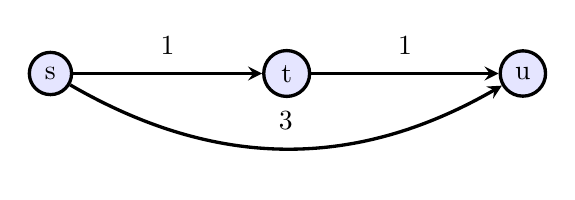
\begin{tikzpicture}[->,>=stealth,node distance=3cm,very
            thick,node/.style={circle,fill=blue!10,draw}]

            \node[node] (s) {s};
            \node[node] (t) [right of=s] {t};
            \node[node] (u) [right of=t] {u};

            \path[every node]

            (s) edge node [above=1mm] {1} (t)
                edge [bend right] node [above=1mm] {3} (u)
            (t) edge node [above=1mm] {1} (u);
        \end{tikzpicture}
        \caption{The graph \(G\).}
        \label{fig:graph1}

        \vspace{.2in}

        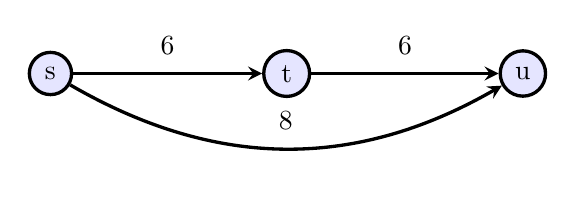
\begin{tikzpicture}[->,>=stealth,node distance=3cm,very
            thick,node/.style={circle,fill=blue!10,draw}]

            \node[node] (s) {s};
            \node[node] (t) [right of=s] {t};
            \node[node] (u) [right of=t] {u};

            \path[every node]

            (s) edge node [above=1mm] {6} (t)
                edge [bend right] node [above=1mm] {8} (u)
            (t) edge node [above=1mm] {6} (u);
        \end{tikzpicture}
        \caption{The graph \(G'\).}
        \label{fig:graph2}
    \end{figure}

\end{homeworkProblem}

\end{document}
